%-------------------------------------------------------------------------------------------------------
%-------------------------------------------------------------------------------------------------------
% Sec & Label

\section{Theoretical Analysis}
\label{sec:analysis}


%-------------------------------------------------------------------------------------------------------
%-------------------------------------------------------------------------------------------------------
% Intro

In this section we will explain the inner workings of the class A audio amplifier created and perform a theoretical analysis of each component. 
The common Kirchoff laws and the simplified BJT equation were used to perform the analysis.

%-----------------------------------------------------------------------
%-----------------------------------------------------------------------
% 		     	    Transf - subsec
% ----------------------------------------------------------------------
% ----------------------------------------------------------------------

\subsection{Gain stage - Degenerated Common Emitter Amplifier}
\label{subsec:transf}



It is in this stage of the amplifier that most of the signal amplification takes place. This stage is comprised of a NPN tansistor, two capacitors (coupling and bypass) and four resistors (two for the voltage divider, $R_1$ and $R_2$, one for the temperature stabilization $R_E$ and another to set the no signal current, $R_C$).

The base voltage of the transistor needs to be forward biased in order for the NPN transistor to work in the forward-active region. For that reason, a voltage divider is added to make sure that the base voltage is always larger than $0.7V$. A coupling capacitor is added between the voltage divider and the signal source in order to add the input AC signal to the voltage divider DC signal (this will be explained in more detail in the simulation section).

The resistor $R_C$ is used to set the zero signal current that passes trough the BJT.

The resistance $R_E$ adds temperature stabilization and removes the temperature dependency of the gain in the circuit but has the drawback of decreasing the AC gain of the amplifier. A bypass capacitor is used to decrease the gain degenerating effects of $R_E$ on higher frequencies (this will be explained in more detail in the simulation section).



By analysis of the circuit using the mesh method, it is possible to find expressions for the input and output impedances of this stage. The derivation of these equations was performed in lecture 16.


Input impedance:
\[
Z_i=\frac{(r_0+R_c+R_E)(R_B+r_{\pi}+R_E) + g_mR_Er_0r_{\pi}-R_E^2}{r_o + R - R_E}
\]


Output impedance:
\[
Z_o=Z_x||R
\]

\[
Z_x=r_0\frac{\frac{1}{R_E}+\frac{1}{r_{pi}+R_B}+\frac{1}{r_o}+\frac{g_mr_{\pi}}{r_{pi}+R_B}}{\frac{1}{R_E}+\frac{1}{r_{pi}+R_B}}
\]

The Common Emitter has the drawback of having high output impedance. For that reason the Output stage is added as way of reducing the output impedance and to suplly more current to the load.

\subsection{Output stage - Common Collector Amplifier}
\label{subsec:envdet}

The output stage is comprised of a PNP transistor, a resistor and a capacitor.


This stage has a gain level of almost unity so it is not responsible for the amplification. The main purpose is to decrease the output impedance to work better with the $8${\emph {Ohm}} load and allow larger currents to flow.


The capacitor is used to remove the DC component of the signal and only allow for the AC signal to reach the output terminals.


By analysis of the circuit using the node methos, it is possible to find expressions for the input and output impedances of this stage. The derivation of these equations was performed in lecture 17.


Input impedance:
\[
Z_i = \frac{g_{\pi}+g_E+g_o+g_m}{g_{\pi}(g_{\pi}+g_E+g_o)}
\]

This value is higher than the output impedance of the gain stage. Since both the stages are connected in series, they follow the voltage divider law. For that reason, to achive as large as possible gain, it is important that the output impedance of the gain stage is smaller than the input impedance of the output stage.

Output impedance:

\[
Z_o = \frac{1}{g_{pi}+g_E+g_o+g_m}
\]

This value is low so it can be connected to the load efficiently.

\subsection {Circuit frequency response}
Due to the use of capacitors in the circuit, the gain is dependent on the frenquecy of the imput. This response was achieved by calculating the equivelent impedance of the braches with capacitors for a set of frequencies.

%\begin{figure}[ht]
%	\centering
%	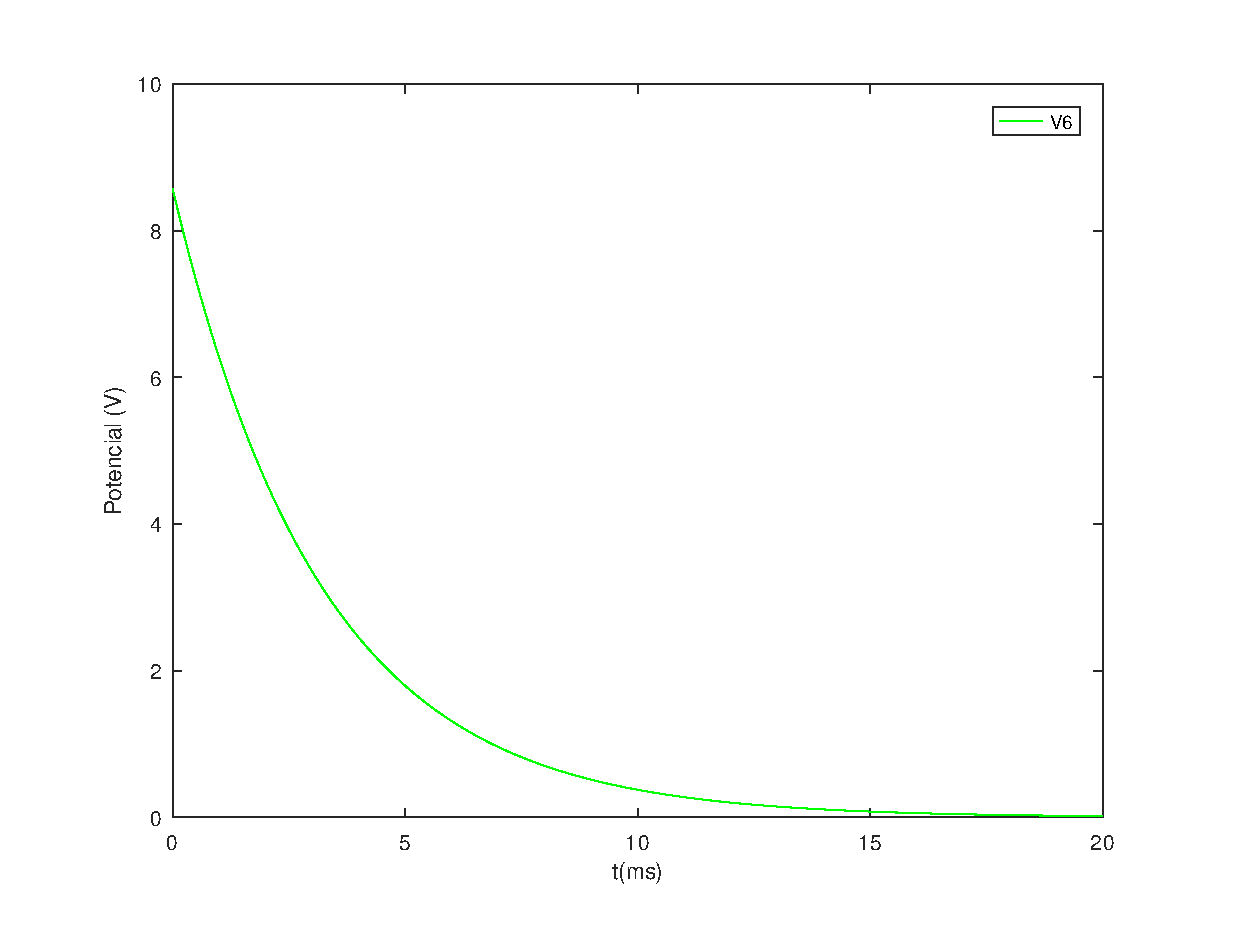
\includegraphics[width=0.7\linewidth]{plot1.eps}
%	\caption{Frequency Response Vo/Vi.}
%\label{fig:oct}
%\end{figure}

%-----------------------------------------------------------------------
%-----------------------------------------------------------------------
% 			     Results - subsec
% ----------------------------------------------------------------------
% ----------------------------------------------------------------------

\subsection{Theoretical Results}
\label{subsec:res_the}

The obtained results were as follows:

%\begin{table}[ht]
%	\centering
%	\begin{tabular}{|l|r|}
%		\hline    
%		{\bf Name} & {\bf Value} \\ \hline
%   		$Ve$ & 1.093271e+00 \\ \hline 
$Vc$ & 9.912854e+00 \\ \hline 
$Vce$ & 8.819583e+00 \\ \hline 
$Vec2$ & 1.061285e+01 \\ \hline 

%	\end{tabular}
%	
%	\caption{Values from Octave.}
%   
%\label{tab:op_teo}
%\end{table}

%\begin{table}[ht]
%	\centering
%	\begin{tabular}{|l|r|}
%		\hline    
%		{\bf Name} & {\bf Value[Ohm]} \\ \hline
%   		$Z1_{In}$ & 8.064050e+03 \\ \hline 
$Z1_{Out}$ & 9.951958e+02 \\ \hline 
$Z2_{In}$ & 8.598855e+03 \\ \hline 
$Z2_{Out}$ & 3.021730e-01 \\ \hline 
$Zt_{Out}$ & 4.411395e+00 \\ \hline 

%	\end{tabular}
%	
%	\caption{Values from Octave.}
%\label{tab:imp_teo}
%\end{table}


